\begin{frame}
	\frametitle{Controlo de pre\c cos: $P_{max}$}
	O Governo fixa compulsivamente um pre\c co abaixo do pre\c co de equil\'ibrio:

	\vspace{0.2cm}

	Pretende impedir que o pre\c co do bem suba acima do pre\c co tabelado, de modo a beneficiar os consumidores (ex.: controlo das rendas)
	
\end{frame}

\begin{frame}
	\frametitle{Pre\c cos M\'aximos}
	\begin{columns}
		\begin{column}{0.6\textwidth}
			\begin{center}
				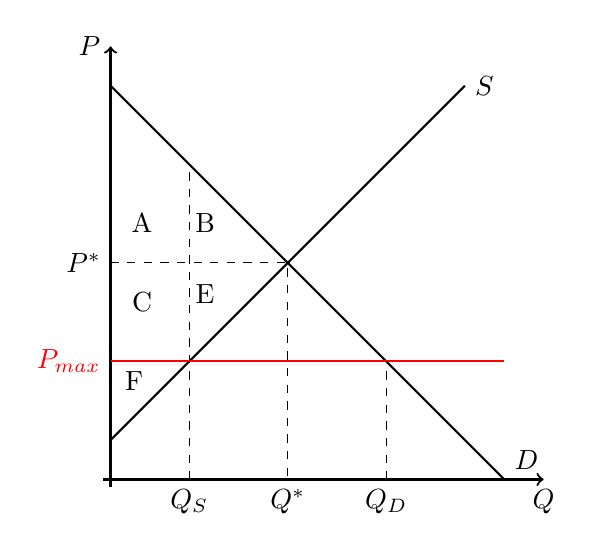
\begin{tikzpicture}[
					scale = 1,
					every node/.style = {scale = 1},
					declare function = {
						d(\x) = 5 - \x;
						s(\x) = 0.5 + \x;
					}]
					\def\eq{9/4}

					\draw[thick,->] (-0.1,0) -- (5.5,0)node[below]{$Q$};
					\draw[thick,->] (0,-0.1) -- (0,5.5)node[left]{$P$};

					\draw[thick,domain=0:5,variable=\x] plot (\x,{d(\x)})node[above right]{$D$};
					\draw[thick,domain=0:4.5,variable=\x] plot (\x,{s(\x)})node[right]{$S$};

					\draw[thick,red] (0,1.5)node[left]{$P_{max}$} -- (5,1.5);
					\draw[dashed] (0,{s(\eq)})node[left]{$P^*$} -- (\eq,{s(\eq)}) -- (\eq,0)node[below]{$Q^*$};

					\draw[dashed] (1,0)node[below]{$Q_S$} -- (1,{d(1)});
					\draw[dashed] (3.5,0)node[below]{$Q_D$} -- (3.5,{d(3.5)});

					\draw(0.4,{d(\eq)+0.5})node[]{A};
					\draw(0.4,{d(\eq)-0.5})node[]{C};
					\draw(0.3,{d(\eq)-1.5})node[]{F};
					\draw(1.2,{d(\eq)+0.5})node[]{B};
					\draw(1.2,{d(\eq)-0.4})node[]{E};

				\end{tikzpicture}
			\end{center}
		\end{column}
		\begin{column}{0.4\textwidth}
			\begin{itemize}
				\item O mercado fica equilibrado?
				\item Qual a altera\c c\~ao ao excedente do consumidor? Continua a ter o mesmo significado?
				\item Qual a altera\c c\~ao no excedente do produtor?
			\end{itemize}
		\end{column}
	\end{columns}
\end{frame}

\begin{frame}
	\frametitle{Pre\c cos M\'aximos: reflex\~ao}
	\begin{enumerate}
		\item Ser\~ao os consumidores que mais valorizam o bem aqueles que o conseguem consumir?
		\item Quais as consequ\^encias da possibilidade de revender o bem?
		\item Estar\~ao os produtores dispostos a apostar na qualidade, num mercado regulado desta maneira?
		\item Como se aplicam as conclus\~oes acima ao mercado imobili\'ario no caso de rendas controladas? (admitindo que n\~ao h\'a falhas de mercado e que a concorr\^encia perfeita \'e uma boa forma de o descrever?)
	\end{enumerate}
\end{frame}

\begin{frame}
	\frametitle{Controlo de Pre\c cos - $P_{min}$}
	O Governo fixa compulsivamente um pre\c co acima do pre\c co de equil\'ibrio
	\begin{itemize}
		\item estabelece um pre\c co limite para que os produtores possam vender o bem (ex.: pre\c co de alguns produtos agr\'icolas). O objectivo \'e, normalmente, beneficiar os produtores.
		\item O sal\'ario m\'inimo \'e um pre\c co m\'inimo estabelecido no mercado do trabalho.
	\end{itemize}
\end{frame}

\begin{frame}
	\frametitle{Pre\c cos M\'inimos}
	\begin{columns}
		\begin{column}{0.6\textwidth}
			\begin{center}
				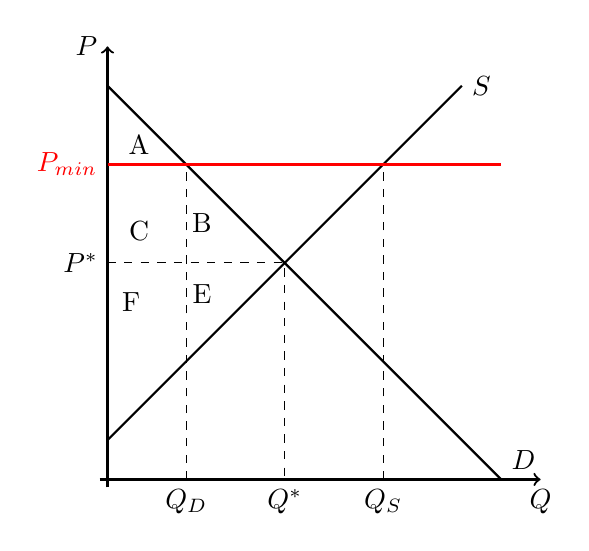
\begin{tikzpicture}[
					scale = 1,
					every node/.style = {scale = 1},
					declare function = {
						d(\x) = 5 - \x;
						s(\x) = 0.5 + \x;
					}]
					\def\eq{9/4}

					\draw[thick,->] (-0.1,0) -- (5.5,0)node[below]{$Q$};
					\draw[thick,->] (0,-0.1) -- (0,5.5)node[left]{$P$};

					\draw[thick,domain=0:5,variable=\x] plot (\x,{d(\x)})node[above right]{$D$};
					\draw[thick,domain=0:4.5,variable=\x] plot (\x,{s(\x)})node[right]{$S$};

					\draw[thick,red] (0,4)node[left]{$P_{min}$} -- (5,4);
					\draw[dashed] (0,{s(\eq)})node[left]{$P^*$} -- (\eq,{s(\eq)}) -- (\eq,0)node[below]{$Q^*$};

					\draw[dashed] (1,0)node[below]{$Q_D$} -- (1,{d(1)});
					\draw[dashed] (3.5,0)node[below]{$Q_S$} -- (3.5,{s(3.5)});

					\draw(0.4,{d(\eq)+1.5})node[]{A};
					\draw(0.4,{d(\eq)+0.4})node[]{C};
					\draw(0.3,{d(\eq)-0.5})node[]{F};
					\draw(1.2,{d(\eq)+0.5})node[]{B};
					\draw(1.2,{d(\eq)-0.4})node[]{E};

				\end{tikzpicture}
			\end{center}
		\end{column}
		\begin{column}{0.4\textwidth}
			\begin{itemize}
				\item O mercado fica equilibrado?
				\item Qual a altera\c c\~ao ao excedente do consumidor?
				\item Qual a altera\c c\~ao no excedente do produtor? Continua a ter o mesmo significado?
			\end{itemize}
		\end{column}
	\end{columns}
\end{frame}

\begin{frame}
	\frametitle{Pre\c cos M\'inimos: reflex\~ao}
	\begin{enumerate}
		\item Ser\~ao os consumidores que mais valorizam o bem aqueles que o conseguem consumir?
		\item Os produtores conseguem escoar todo o seu stock?
		\item O que poder\'a ser feito para evitar acumula\c c\~ao de stocks e manter o pre\c co alto?
		\item Haver\'a efici\^encia na utiliza\c c\~ao de recursos?
		\item Como se aplicam as conclus\~oes acima ao mercado do trabalho com o sal\'ario m\'inimo (admitindo que n\~ao h\'a falhas de mercado e que a concorr\^encia perfeita \'e uma boa forma de o descrever)
	\end{enumerate}
\end{frame}